\section{mechanical design and prototype development}

The robotic arm is designed with 5 DOF that has a working dimension which is similar to a human arm and it is capable of grasping an object along a predefined trajectory. The mechanical design of it was considered to develop a suitable structure capable of performing the pick-and-place operation. The design process initially focused on determining the required degrees of freedom, joint movements, workspace and arrangement of the robotic arm links. 

\subsection{Mechanical Design Concept}

The main mechanical design concept is focused on five degrees of freedom that allow the arm to perform coordinated movements through its different joints and position the end effector at the required locations within its intended workspace. The lengths and orientations of the links were determined according to the required movements to provide sufficient reach for the intended pick-and-place task. 

\subsection{SolidWorks CAD Modeling}

The three-dimensional CAD model of this robotic arm was developed using SolidWorks 2022 software. All mechanical components and parts were designed individually and then combined them to form the complete robotic arm assembly. All these links, joints and the structure were designed according to the predefined dimensions and mechanical constraints which were required for the desired application. This model provides a visual representation of the proposed mechanical structure. It was used to support the evaluation of the initial design before going to the physical prototype.

\begin{figure}[htbp]
    \centering
    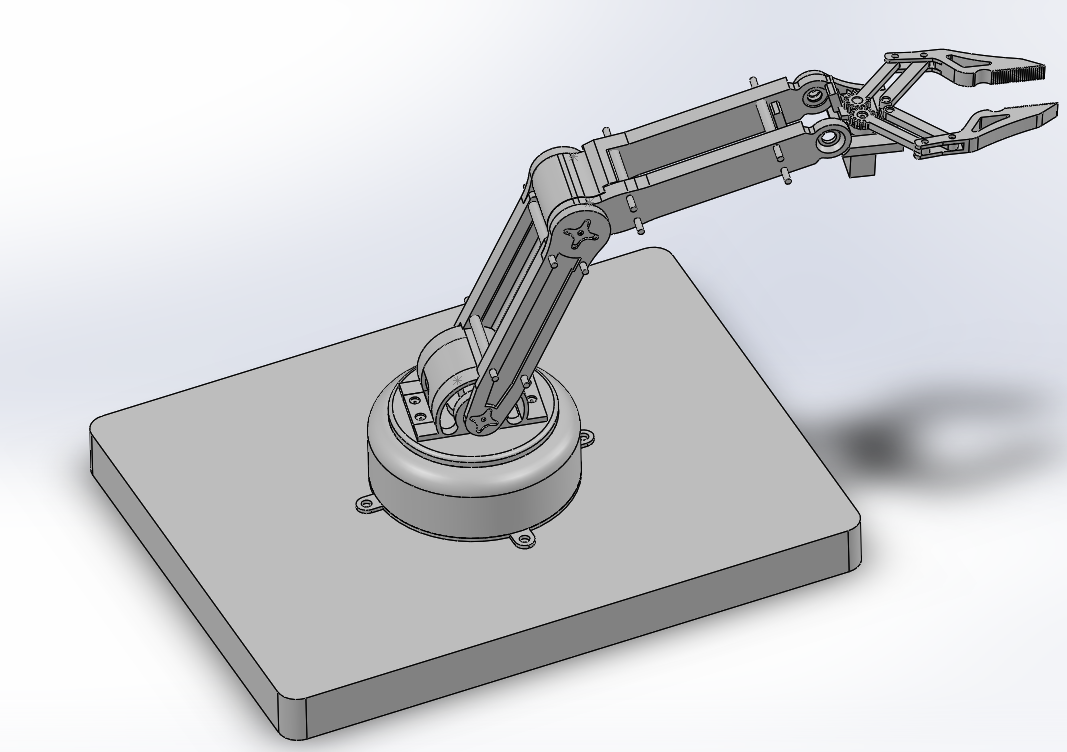
\includegraphics[width=\columnwidth]{figures/solidworks design.png}
    \caption{3D model of the proposed 5-DOF robotic arm}
    \label{fig:Solid design}
\end{figure}

\subsection{Final Prototype Structure Selection}

A metal robotic arm structure was used for the final prototype due to the practical requirements of fabrication and implementation of the initial robotic arm structure which was designed using SolidWorks. This arm structure was selected to reduce fabrication complexity, accelerate the implementation process and increase the reliability of the system. It was adapted to accommodate the required servo motors, gripper mechanism and object detection sensor which maintains the required five-degree-of-freedom configuration.  

\subsection{Final Mechanical Assembly}

The final mechanical assembly of this system consists, arm structure, servo motors, gripper mechanism and sensor mounting arrangement. Each servo motor is installed at the corresponding joints to provide controlled movement of the structure during the pick-and-place operation. Gripper mechanism is used for grasping and releasing the object in the right positions and it is mounted at the end effector. The sensor mounting system was designed to correctly detect the object while avoiding interference with the movement of the robotic arm. This final mechanical assembly was checked to ensure that the robotic arm could perform the required movements for the pick-and-place operation.

\begin{figure}[htbp]
    \centering
    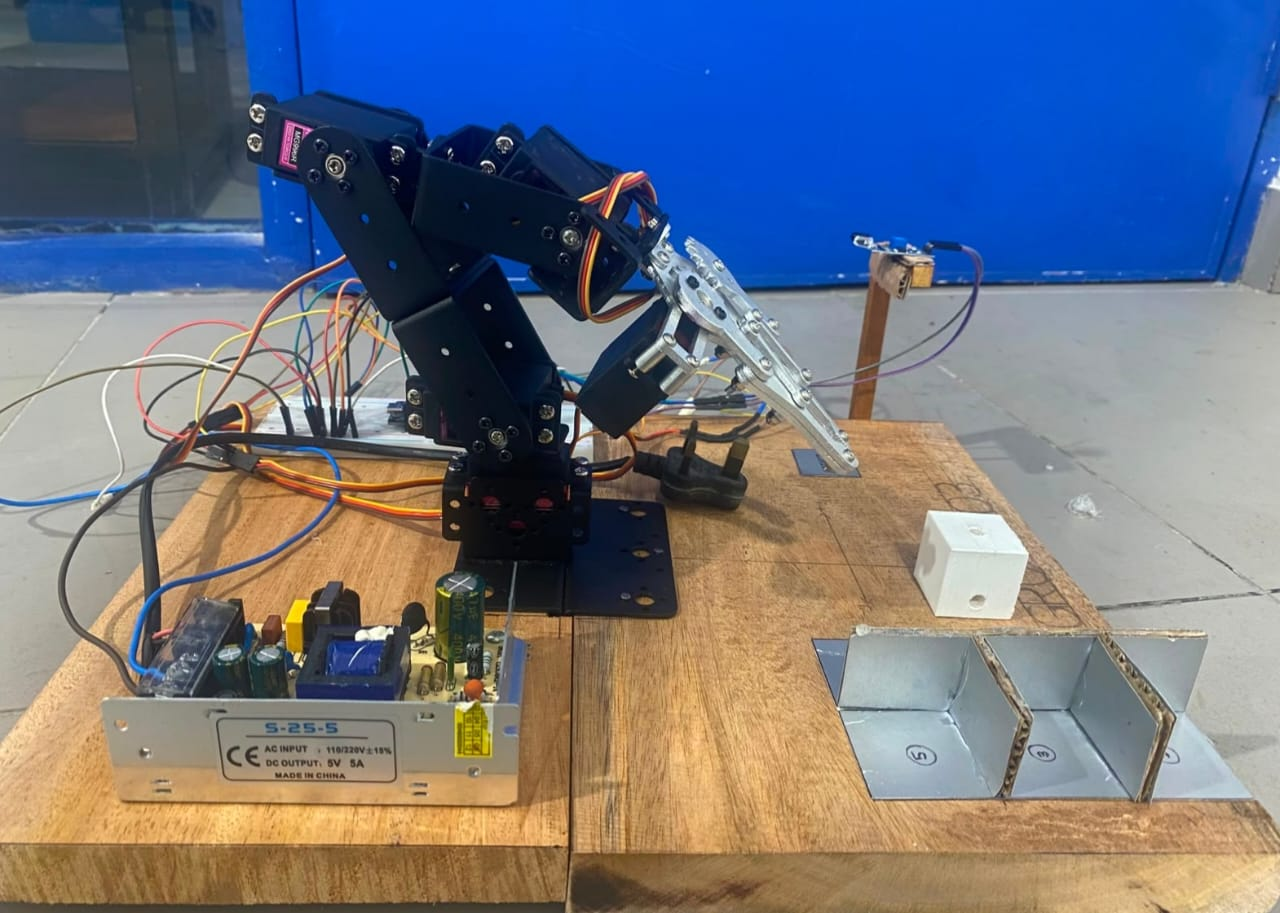
\includegraphics[width=\columnwidth]{figures/final assembly.jpeg}
    \caption{Final assembled prototype of the developed robotic arm}
    \label{fig:assembly}
\end{figure}


